\documentclass[14pt]{extbook}
\usepackage{multicol, enumerate, enumitem, hyperref, color, soul, setspace, parskip, fancyhdr} %General Packages
\usepackage{amssymb, amsthm, amsmath, latexsym, units, mathtools} %Math Packages
\everymath{\displaystyle} %All math in Display Style
% Packages with additional options
\usepackage[headsep=0.5cm,headheight=12pt, left=1 in,right= 1 in,top= 1 in,bottom= 1 in]{geometry}
\usepackage[usenames,dvipsnames]{xcolor}
\usepackage{dashrule}  % Package to use the command below to create lines between items
\newcommand{\litem}[1]{\item#1\hspace*{-1cm}\rule{\textwidth}{0.4pt}}
\pagestyle{fancy}
\lhead{Progress Quiz 8}
\chead{}
\rhead{Version A}
\lfoot{5493-4176}
\cfoot{}
\rfoot{Summer C 2021}
\begin{document}

\begin{enumerate}
\litem{
Choose the graph of the equation below.\[ f(x) = \frac{-1}{x + 2} - 2 \]\begin{enumerate}[label=\Alph*.]
\begin{multicols}{2}\item 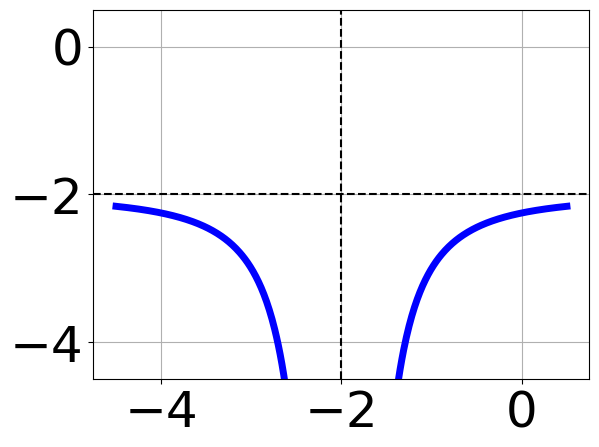
\includegraphics[width = 0.3\textwidth]{../Figures/rationalEquationToGraphCopyAA.png}\item 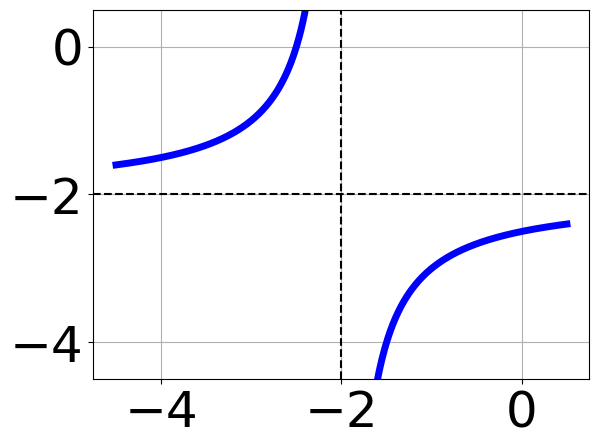
\includegraphics[width = 0.3\textwidth]{../Figures/rationalEquationToGraphCopyBA.png}\item 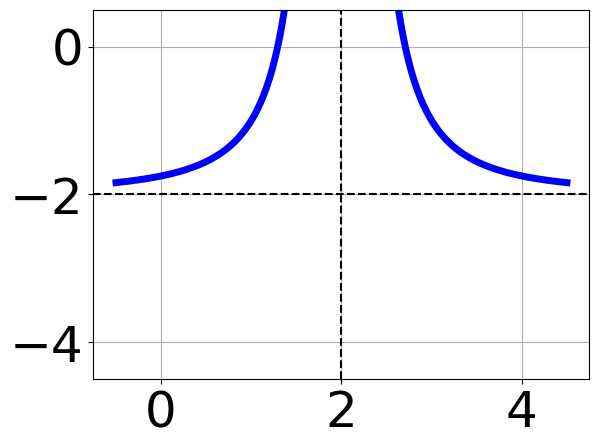
\includegraphics[width = 0.3\textwidth]{../Figures/rationalEquationToGraphCopyCA.png}\item 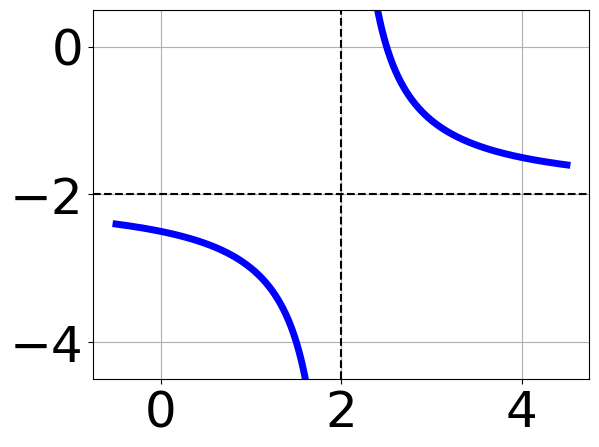
\includegraphics[width = 0.3\textwidth]{../Figures/rationalEquationToGraphCopyDA.png}\end{multicols}\item None of the above.
\end{enumerate} }
\litem{
Solve the rational equation below. Then, choose the interval(s) that the solution(s) belongs to.\[ \frac{63}{54x + 27} + 1 = \frac{63}{54x + 27} \]\begin{enumerate}[label=\Alph*.]
\item \( x \in [-0.5,0.5] \)
\item \( x_1 \in [-1.5, 0.2] \text{ and } x_2 \in [0.3,1.4] \)
\item \( x_1 \in [-1.5, 0.2] \text{ and } x_2 \in [-1.4,0.1] \)
\item \( \text{All solutions lead to invalid or complex values in the equation.} \)
\item \( x \in [0.3,0.8] \)

\end{enumerate} }
\litem{
Choose the graph of the equation below.\[ f(x) = \frac{1}{(x - 1)^2} + 3 \]\begin{enumerate}[label=\Alph*.]
\begin{multicols}{2}\item 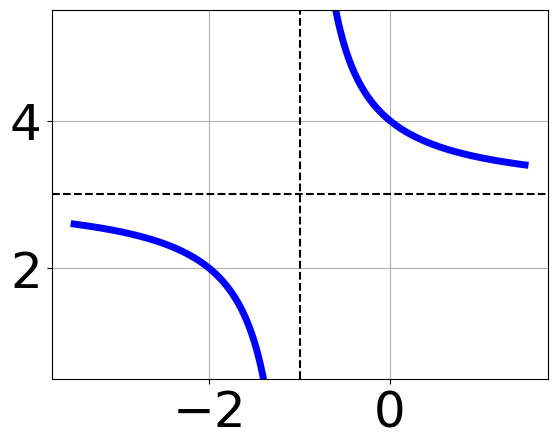
\includegraphics[width = 0.3\textwidth]{../Figures/rationalEquationToGraphAA.png}\item 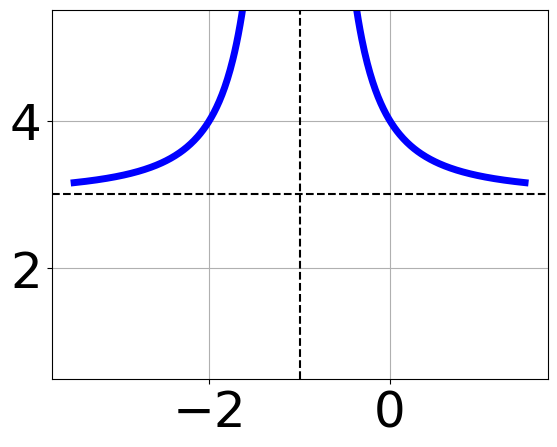
\includegraphics[width = 0.3\textwidth]{../Figures/rationalEquationToGraphBA.png}\item 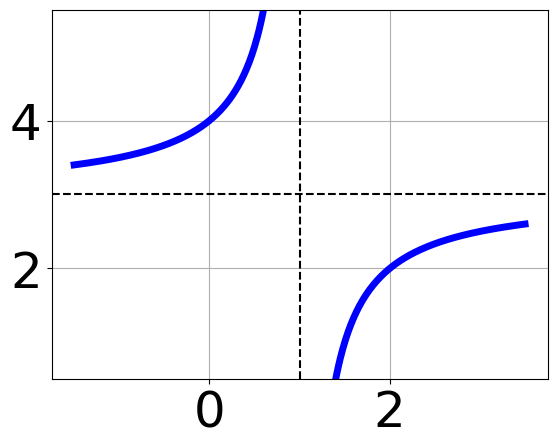
\includegraphics[width = 0.3\textwidth]{../Figures/rationalEquationToGraphCA.png}\item 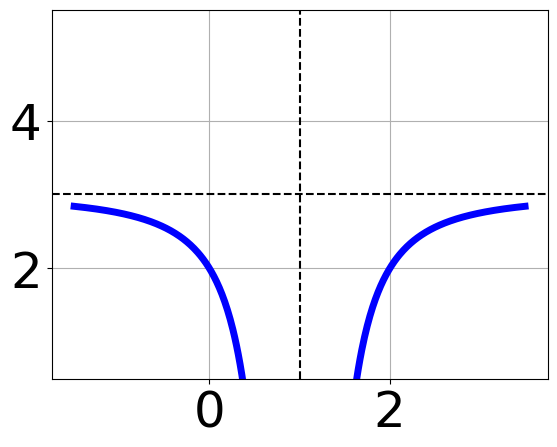
\includegraphics[width = 0.3\textwidth]{../Figures/rationalEquationToGraphDA.png}\end{multicols}\item None of the above.
\end{enumerate} }
\litem{
Solve the rational equation below. Then, choose the interval(s) that the solution(s) belongs to.\[ \frac{-6}{-6x -4} + -8 = \frac{8}{48x + 32} \]\begin{enumerate}[label=\Alph*.]
\item \( x \in [-2.56,1.44] \)
\item \( x_1 \in [-1.3, 0.4] \text{ and } x_2 \in [0.77,1.77] \)
\item \( \text{All solutions lead to invalid or complex values in the equation.} \)
\item \( x_1 \in [-1.3, 0.4] \text{ and } x_2 \in [-1.38,0.62] \)
\item \( x \in [0.2,1] \)

\end{enumerate} }
\litem{
Determine the domain of the function below.\[ f(x) = \frac{6}{15x^{2} -8 x -16} \]\begin{enumerate}[label=\Alph*.]
\item \( \text{All Real numbers except } x = a \text{ and } x = b, \text{ where } a \in [-20, -18] \text{ and } b \in [10, 15] \)
\item \( \text{All Real numbers except } x = a, \text{ where } a \in [-0.8, 1.2] \)
\item \( \text{All Real numbers except } x = a, \text{ where } a \in [-20, -18] \)
\item \( \text{All Real numbers except } x = a \text{ and } x = b, \text{ where } a \in [-0.8, 1.2] \text{ and } b \in [0.33, 5.33] \)
\item \( \text{All Real numbers.} \)

\end{enumerate} }
\litem{
Solve the rational equation below. Then, choose the interval(s) that the solution(s) belongs to.\[ \frac{-2x}{6x -7} + \frac{-3x^{2}}{24x^{2} +8 x -42} = \frac{-6}{4x + 6} \]\begin{enumerate}[label=\Alph*.]
\item \( \text{All solutions lead to invalid or complex values in the equation.} \)
\item \( x_1 \in [3.5, 4.4] \text{ and } x_2 \in [-1.22,3.78] \)
\item \( x_1 \in [0.1, 1.4] \text{ and } x_2 \in [-6.5,0.5] \)
\item \( x \in [-3.7,0.3] \)
\item \( x \in [0.1,1.4] \)

\end{enumerate} }
\litem{
Determine the domain of the function below.\[ f(x) = \frac{5}{18x^{2} +15 x -25} \]\begin{enumerate}[label=\Alph*.]
\item \( \text{All Real numbers except } x = a \text{ and } x = b, \text{ where } a \in [-17, -13] \text{ and } b \in [29, 32] \)
\item \( \text{All Real numbers.} \)
\item \( \text{All Real numbers except } x = a, \text{ where } a \in [-3.67, -0.67] \)
\item \( \text{All Real numbers except } x = a, \text{ where } a \in [-17, -13] \)
\item \( \text{All Real numbers except } x = a \text{ and } x = b, \text{ where } a \in [-3.67, -0.67] \text{ and } b \in [0.83, 3.83] \)

\end{enumerate} }
\litem{
Solve the rational equation below. Then, choose the interval(s) that the solution(s) belongs to.\[ \frac{-3x}{-2x + 6} + \frac{-2x^{2}}{12x^{2} -48 x + 36} = \frac{5}{-6x + 6} \]\begin{enumerate}[label=\Alph*.]
\item \( x \in [1.34,1.87] \)
\item \( x_1 \in [-1.15, -0.96] \text{ and } x_2 \in [3,6] \)
\item \( x \in [0.46,1.62] \)
\item \( \text{All solutions lead to invalid or complex values in the equation.} \)
\item \( x_1 \in [-1.15, -0.96] \text{ and } x_2 \in [-2.36,2.64] \)

\end{enumerate} }
\litem{
Choose the equation of the function graphed below.
\begin{center}
    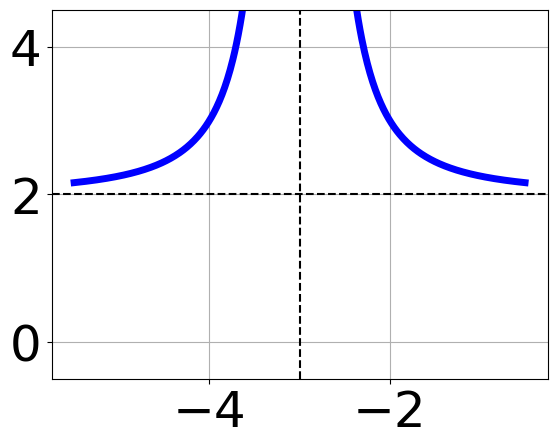
\includegraphics[width=0.5\textwidth]{../Figures/rationalGraphToEquationA.png}
\end{center}
\begin{enumerate}[label=\Alph*.]
\item \( f(x) = \frac{-1}{(x + 3)^2} + 2 \)
\item \( f(x) = \frac{-1}{x + 3} + 2 \)
\item \( f(x) = \frac{1}{(x - 3)^2} + 2 \)
\item \( f(x) = \frac{1}{x - 3} + 2 \)
\item \( \text{None of the above} \)

\end{enumerate} }
\litem{
Choose the equation of the function graphed below.
\begin{center}
    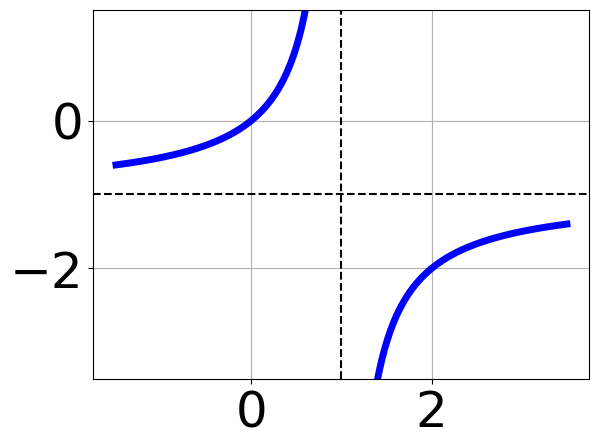
\includegraphics[width=0.5\textwidth]{../Figures/rationalGraphToEquationCopyA.png}
\end{center}
\begin{enumerate}[label=\Alph*.]
\item \( f(x) = \frac{1}{x + 1} - 1 \)
\item \( f(x) = \frac{-1}{(x - 1)^2} - 1 \)
\item \( f(x) = \frac{-1}{x - 1} - 1 \)
\item \( f(x) = \frac{1}{(x + 1)^2} - 1 \)
\item \( \text{None of the above} \)

\end{enumerate} }
\end{enumerate}

\end{document}